% Ich teile hier einfach mal meine Erfahrung der letzten Stunde trouble shooting.
% Latex = alles gut
% Bibtex = Denk einfach nich daran Umlaute zu benutzen. Nicht in der Bibliography, und auch nicht in Dateinamen
% Im eigentlichen Text gehts. Sachen wie Carrá sind aus irgendeinem Grund wiederum erlaubt, auch in der Bibliography
% Fix: {\"o} statt ö etc. (inkl. eckigen Klammern)

\chapter{Einführung}
\begin{itemize}
\item Wie funktionieren Unternehmen und Prozesse aktuell?
\item Wie sieht die typische Unternehmenskultur aus und welche Nachteile bringt sie mit sich? (vllt auch Vorteile, weil mir wollen ja sachlich ran gehen)
	\begin{itemize}
	\item Silodenken
	\item Wall of Confusion
	\end{itemize}
\item Warum braucht es etwas Neues?
\item (optional) Andere Ansätze die das selbe Problem angegangen sind (bzw. andere Modelle für Unternehmenskultur)?
\end{itemize}

\begin{figure}[h]
\centering
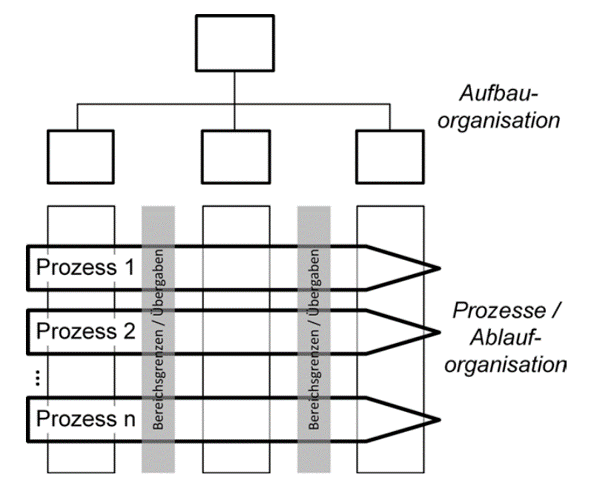
\includegraphics[width=0.7\textwidth]{Graphics/silodenken}
\caption{Silodenken \cite{halstenberg:2020}}
\end{figure}

\begin{figure}[h]
\centering
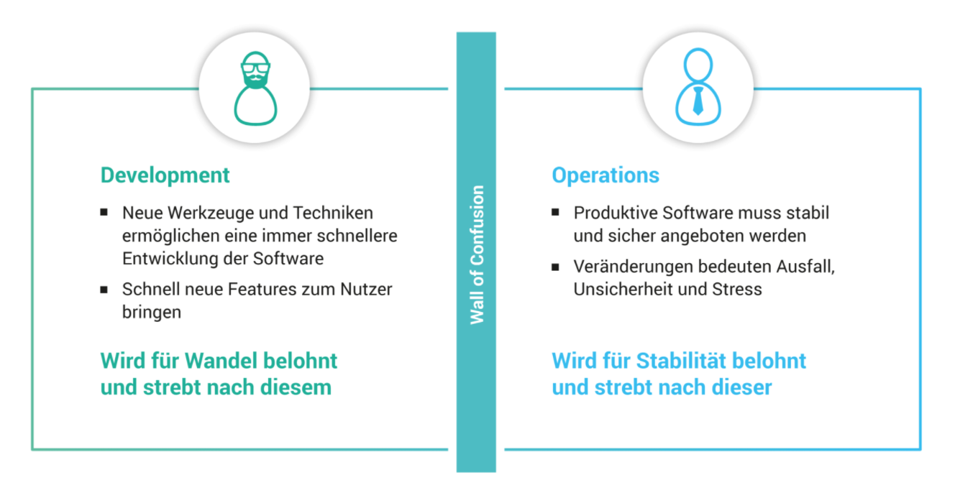
\includegraphics[width=0.8\textwidth]{Graphics/wall_of_confusion}
\caption{Wall Of Confusion \cite{novatec:2021}}
\end{figure}
